\documentclass{article}
\usepackage[dvips]{graphicx}
\usepackage{float}
\usepackage{graphics} 
\usepackage{graphicx}
\usepackage{color}
\usepackage{subfig}
%\usepackage[subnum]{cases}
\usepackage{amsmath}
\usepackage{amsthm}
\usepackage{amsfonts}
\usepackage{pifont}
\usepackage{rotating}
\usepackage{latexsym}
\usepackage{verbatim}
%\usepackage[latin1]{inputenc}
\usepackage{multirow}
\usepackage{afterpage}
\usepackage{epsfig}
\usepackage{lscape}
\usepackage{makeidx}
\usepackage{tikz}
\usetikzlibrary{shapes,arrows,positioning,backgrounds,calc,petri,calc,fit}
%\tikzstyle{comp} = [draw, fill=blue!20, rectangle, minimum height=7mm, minimum width=14mm]
\tikzstyle{comp} = [draw, rectangle, minimum height=7mm, minimum width=14mm]
%\tikzstyle{voter} = [draw, fill=blue!20, circle, minimum height=7mm, minimum width=7mm]
\tikzstyle{voter} = [draw, circle, minimum height=7mm, minimum width=7mm]
%\tikzstyle{ftreeevent} = [draw, fill=blue!20, ellipse, minimum height=7mm, minimum width=14mm]
\tikzstyle{ftreeevent} = [draw, ellipse, minimum height=7mm, minimum width=14mm]
%\tikzstyle{state} = [draw, fill=blue!20, circle, minimum height=7mm, minimum width=7mm]
\tikzstyle{state} = [draw, circle, minimum height=7mm, minimum width=7mm]
%\tikzstyle{statebig} = [draw, fill=blue!20, circle, minimum height=11mm, minimum width=11mm]
\tikzstyle{statebig} = [draw, circle, minimum height=11mm, minimum width=11mm]
%[state/.style={circle,draw,thick,minimum size=5mm, node distance=2cm and 2cm}]

\tikzset{imtransition/.style={rectangle,draw=black,fill=black,thick,inner sep=0pt,minimum height=5mm,minimum width=0.05mm}}
\tikzset{every place/.style={minimum size=5mm,thick}}
\tikzset{every transition/.style={thick,draw=black,fill=black,minimum height=5mm,minimum width=0.5mm}}
%\tikzset{transitionr/.style={rectangle,thick,draw=black,fill=black,minimum width=5mm,minimum height=0.05mm}}
\tikzset{transitionr/.style={rectangle,draw=black,fill=black,thick,inner sep=0pt,minimum height=1mm,minimum width=5mm}}
\tikzset{every label/.style= black}
\graphicspath{{./Figures/}}
%
\title{Dependability Analysis of Two Candidate\\ Architectures for a Brake-By-Wire System \\
\vspace{2.0cm}
\small Laboratory report in \\ EDA122 Fault-Tolerant Computer Systems \\[5ex]} % Title
\vspace{2.0cm}
\vfill
\author{Henrik Hugo\\ Lucas Wiman\\ \small Tuesday 17-21 F\\
\vspace{5.0cm}
\\ \small Chalmers University of Technology \\
\small Gothenburg, Sweden 2014\\
\small Version no.: 0.1\\
} % Author name


\begin{document}

\maketitle % Insert the title, author and date
%
%\setlength\parindent{0pt} % Removes all indentation from paragraphs
%
%\renewcommand{\labelenumi}{\alph{enumi}.} % Make numbering in the enumerate environment by letter rather than number (e.g. section 6)
\newpage
\tableofcontents

\newpage
\section{Introduction}
/{This section shall introduce the reader to the subject addressed by the report. It should include i) a brief explanation of how a brake-by-wire system works and its main advantages and drawbacks compared to existing brake systems, and ii) a description of the purpose of the report, i.e., a formulation of the problem to which the report provides an answer. The last paragraph should consist of a “roadmap” of the report.}/
\begin{figure}[h!]
  \centering
  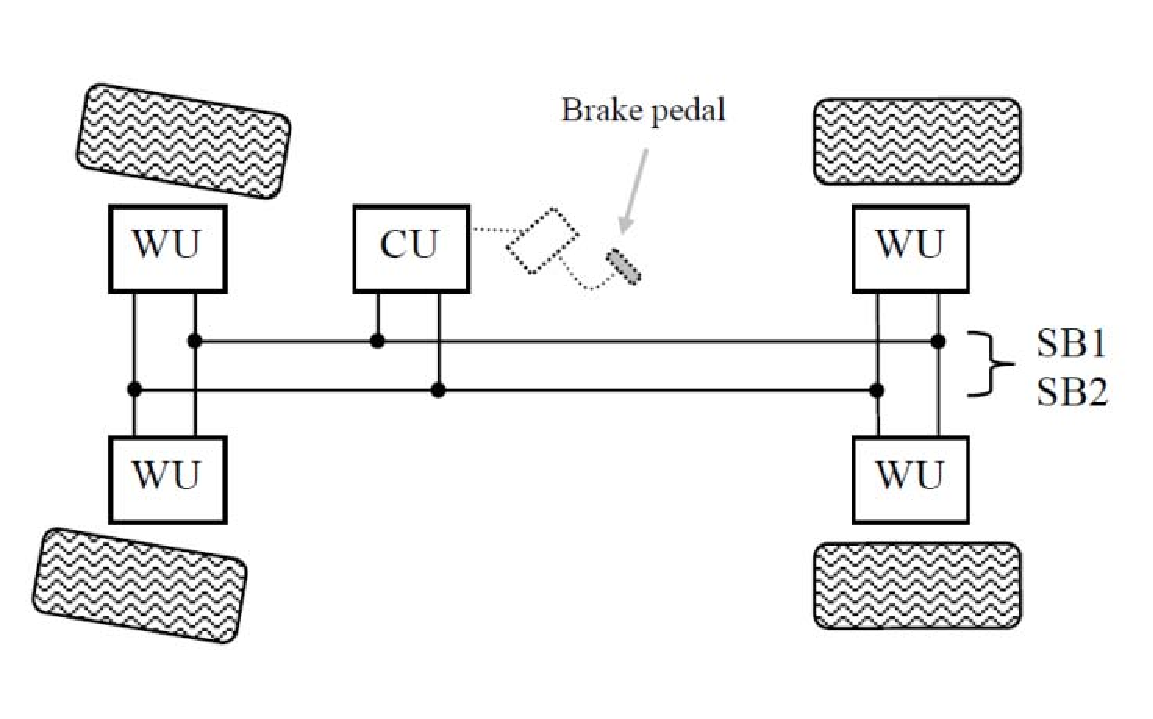
\includegraphics[scale=.5]{Fig1.pdf}
  \caption{Brake-by-wire system}
  \label{fig1}
\end{figure}

%----------------------------------------------------------------------------------------
%	SECTION 2
%----------------------------------------------------------------------------------------
\newpage
\section{Overview of the Candidate Architecture}
The system used in this laboration is implemented in either two configurations; centralized and distributed architectures. There are also two modes of operation which will be taken into consideration for the two architectures, namely full and degraded functionality. Assumptions and modeling parameters for the two architectures described below apply to their respective configurations. 

\subsection{Centralized Architecture}
The centralized architecture relies heavily on the Central Unit (CU) to execute the control algorithm. The wheel units only contain sensors and actuators communicating with the CU over the communication network. With this approach the wheel units contain less hardware and become less complex, leading to lower failure rates in the wheel units. However, the central unit is more complex in this architecture since it requires more processing power and memory, which results in a higher failure rate of the central unit.\\
\\
\subsection{Distributed Architecture}
In comparsion to the Centralized architecture, the distributed architecture instead relies on executing the control algorithm locally for each wheel unit. In addition, for this architecture the wheel units are more complex than in the centralized architecture. The wheel units are similar to the central unit in terms of complexity but suffers from a higher failure rate than the central unit since they are more vulnerable to vibrations, moisture and temperature cycling. 
\subsubsection{Full Functionality}
The system uses two modes of operation which will be analyzed in this report.
The first mode of operation is full functionality which is the standard mode of operation for the system. In order to provide full functionality for the system, the central unit, all four wheel units and at least one system bus must be operational.
\subsubsection{Degraded Functionality}
The second mode of operation is degraded functionality. In this mode, the system can no longer issue the brake command for one of the wheels. As a result, the system is only considered operational if three wheel units, the central unit and at least one system bus are operational. In order to simplify the analysis, the system is considered to have failed catastrophicly
if the system is unable to send its brake command to two or more wheels.
\subsection{Assumptions and modeling parameters}
The table below holds the assumed failure rate of the modules in the brake-by-wire system and their coverage for the centralized architecture and respectively the distributed architecture.  
\begin{table}[h]
\centering
\begin{tabular}{| c | c | c | c |}
\hline 
Subsystem & Part & Failure rate & Coverage\\
\hline
System bus & Serial bus& $5*10^{-7}$ & 1\\
\hline
Wheel unit & Computer module & $15*10^{-6}$ & 1\\
\hline
Wheel unit & Sensor & $2*10^{-6}$ & 1\\
\hline
Wheel unit & Actuator & $1*10^{-6}$ & 1\\
\hline
Central unit & Computer module & $8*10^{-6}$ & 0.99\\
\hline
\end{tabular}
\caption{Failure rates and coverage factors for the distributed architecture}
\label{tab:Put a Lable}
\end{table}
\begin{table}[h]
\centering
\begin{tabular}{| c | c | c | c |}
\hline 
Subsystem & Part & Failure rate & Coverage\\
\hline
System bus & Serial bus& $5*10^{-7}$ & 1\\
\hline
Wheel unit & Computer module & $10*10^{-6}$ & 1\\
\hline
Wheel unit & Sensor & $2*10^{-6}$ & 1\\
\hline
Wheel unit & Actuator & $1*10^{-6}$ & 1\\
\hline
Central unit & Computer module & $10*10^{-6}$ & First CM failure:1 Second CM failure: 0.99\\
\hline
\end{tabular}
\caption{Failure rates and coverage factors for the Centralized Architecture}
\label{tab:Put a Lable}
\end{table}

\newpage
\section{Description of Models}
/{This section shall describe your models for the different subsystems for the two architectures and the two levels of functionality. Figures should be explained in the text.}/

\subsection{Wheel Unit Model}
\begin{figure}[H]
  \centering
  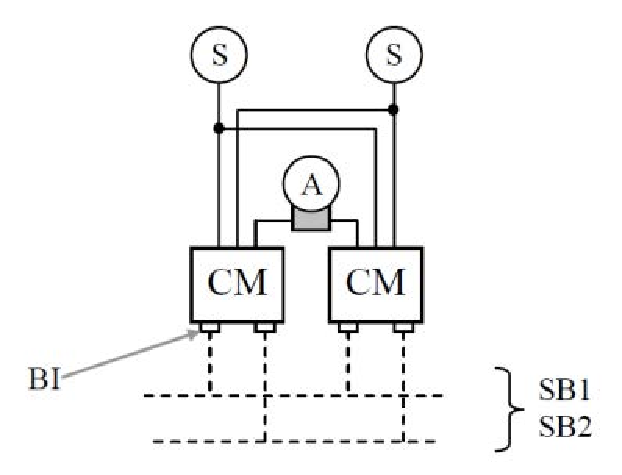
\includegraphics[scale=0.7]{Fig2.pdf}
  \caption{Wheel Unit}
  \label{fig2}
\end{figure}
\begin{figure}[H]
  \centering
  
\includegraphics[scale=1]{Fig3.pdf}
  \caption{Reliability block diagram of the wheel unit}
  \label{fig3}
\end{figure}
%--------------------------------
\subsection{Wheel Unit Subsystem Model}
/text/
\begin{figure}[H]
  \centering
  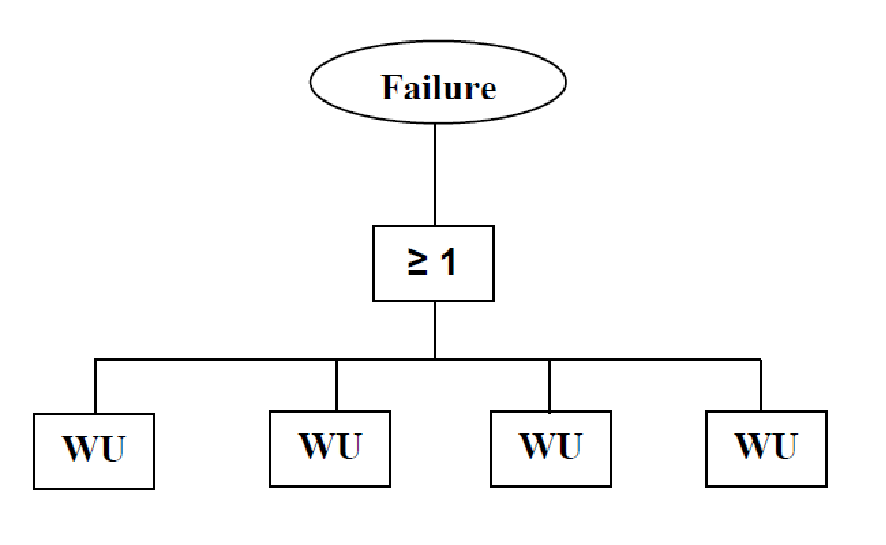
\includegraphics[scale=0.5]{Fig4.pdf}
  \caption{Fault tree for the Wheel Unit Subsystem, full functionality}
  \label{fig4}
\end{figure}
\begin{figure}[H]
  \centering
  
\includegraphics[scale=0.5]{Fig5.pdf}
  \caption{Fault tree for the Wheel Unit Subsystem, degraded functionality}
  \label{fig5}
\end{figure}
%--------------------------------
\subsection{Central Unit (CU)}
\subsubsection{Distributed Duplex Architecture}
\begin{figure}[H]
  \centering
  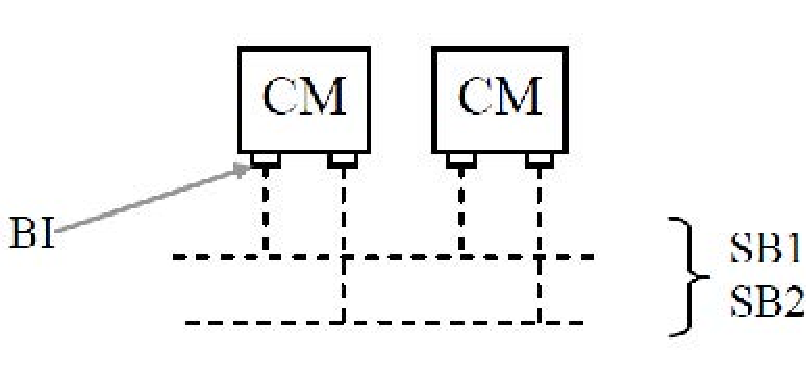
\includegraphics[scale=.5]{Fig6.pdf}
  \caption{Central Unit, duplex configuration }
  \label{fig6}
\end{figure}
\begin{figure}[H]
  \centering
  
\includegraphics[scale=.5]{Fig7.pdf}
  \caption{Reliability block diagram for the Central Unit, duplex configuration}
  \label{fig7}
\end{figure}
%The markov model for central unit-duplex is given below as an example. 
%\begin{figure}[h!]
%  \centering
%  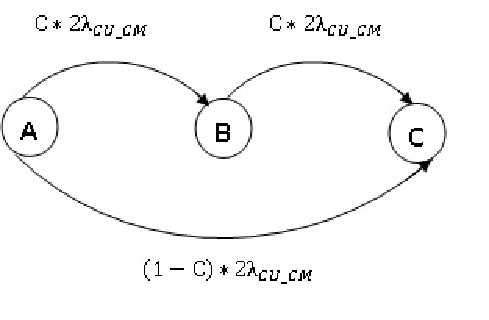
\includegraphics[scale=.7]{Fig8.pdf}
%  \caption{Markov model for the Central Unit. duplex configuration}
%  \label{fig8}
%\end{figure}
\begin{figure}[h!]
\begin{center}
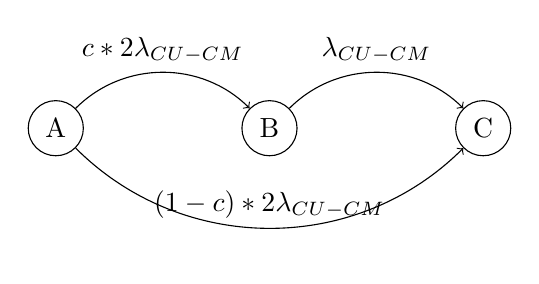
\begin{tikzpicture}[node distance=5mm and 20mm]
\node[state] (s2) {A};
\node[state] (s3) [right= of s2] {B};
\node[state] (s4) [right= of s3] {C};
\draw [->,bend left=45] (s2) to node[above] {$c*2\lambda_{CU-CM} $} (s3);
\draw [->,bend right=45] (s2) to node[above] {$(1-c)*2\lambda_{CU-CM}$} (s4);
\draw [->,bend left=45] (s3) to node[above] {$\lambda_{CU-CM}$} (s4);
\end{tikzpicture}
\caption{Markov chain model}
\end{center}
\end{figure}
%-------------
\subsubsection{Centralized Triplex Architecture}

\begin{figure}[H]
  \centering
  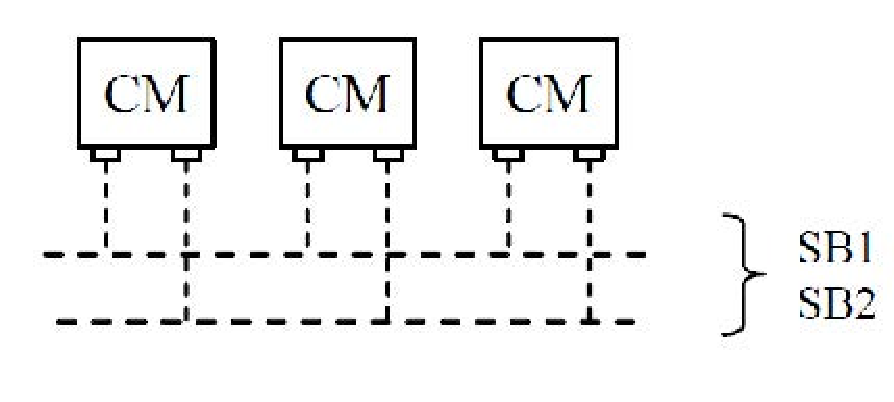
\includegraphics[scale=.5]{Fig9.pdf}
  \caption{Central Unit, triplex configuration }
  \label{fig9}
\end{figure}
/{Reliability block diagram for …, Figure 10.  Make sure the caption number is correct.}/
\\/{Markov model for …, Figure 11.}/

\begin{figure}[H]
  \centering
  
\includegraphics[scale=.5]{Fig10.pdf}
  \caption{Caption }
  \label{fig10}
\end{figure}
\begin{figure}[H]
  \centering
  
\includegraphics[scale=.5]{Fig11.pdf}
  \caption{Caption}
  \label{fig11}
\end{figure}
%--------------------------------
\subsection{System Model}
\subsubsection{Centralized Architecture}

\begin{figure}[H]
  \centering
  
\includegraphics[scale=.5]{Fig12.pdf}
  \caption{Fault tree for Full Functionality}
  \label{fig12}
\end{figure}
\begin{figure}[H]
  \centering
  
\includegraphics[scale=.5]{Fig13.pdf}
  \caption{Fault tree for Degraded Functionality}
  \label{fig13}
\end{figure}
%-------------
\subsubsection{Distributed Architecture}
\begin{figure}[H]
  \centering
  
\includegraphics[scale=.5]{Fig14.pdf}
  \caption{Fault tree for Full Functionality}
  \label{fig14}
\end{figure}
\begin{figure}[H]
  \centering
  
\includegraphics[scale=.5]{Fig15.pdf}
  \caption{Fault tree for Degraded Functionality}
  \label{fig15}
\end{figure}
\newpage
\section{Results}
/{Describe the results. Graphs and tables shall be commented in text. To facilitate the comparison of the results for different design solutions, include several reliability graphs in one diagram.}/
\begin{table}[h]
\centering
\begin{tabular}{| c | c | c |}
\hline
Units&Distributed&Centralized\\
\hline
\multirow{2}{*}{Wheel Unit Subsystem Full Functionality} & Reliability= &Reliability= \\
 & MTTF= & MTTF= \\
\hline
\multirow{2}{*}{Wheel Unit Subsystem Degraded Functionality}& Reliability= &Reliability= \\
 & MTTF= & MTTF= \\
\hline
\multirow{2}{*}{Central Unit}& Reliability= &Reliability= \\
 & MTTF= & MTTF= \\
\hline
\multirow{2}{*}{Entire System Full Functionality}& Reliability= &Reliability= \\
 & MTTF= & MTTF= \\
\hline
\multirow{2}{*}{Entire System Degraded Functionality}& Reliability= &Reliability= \\
 & MTTF= & MTTF= \\
\hline
\end{tabular}
\caption{Reliability and MTTF results}
\label{tab:Put a Lable}
\end{table}
\\/{Insert Reliability Graphs and comment them in the text. Make sure that the caption numbers are correct.}/
\newpage
\section{Discussion}
/{Discuss the pros and cons of the different design solutions.} /

\newpage
\section{Conclusions}
/{Present your conclusions and recommendations.}/
\addcontentsline{toc}{section}{References}

\begin{thebibliography}{9}
%\bibitem{lamport94}
%  Leslie Lamport,
%  \emph{\LaTeX: A Document Preparation System}.
%  Addison Wesley, Massachusetts,
%  2nd Edition,
%  1994.

Please use Vancouver/IEEE style for your referencing. For more information please check: http://www.lib.unimelb.edu.au/cite/ieee/index.html
\\
The reference list shall be formatted as the reference list in this document. For an example of how to write references, see Kopetz and Bauer [1]. (This paper is part of the course literature and is published by the Institute of Electrical and Electronics Engineers, Inc, known as IEEE, and therefore follows the IEEE format for scientific journal papers. Other publishers use slightly different formats.)

\end{thebibliography}


\end{document}
